\documentclass [xcolor=svgnames, t] {beamer} 
\usepackage[utf8]{inputenc}
\usepackage{booktabs, comment} 
\usepackage[absolute, overlay]{textpos} 
\usepackage{pgfpages}
\usepackage[font=footnotesize]{caption}
\useoutertheme{infolines} 
\usepackage{advdate}
\definecolor{gold}{RGB}{254, 206, 0}

\setbeamercolor{title in head/foot}{bg=gray, fg=black}
\setbeamercolor{author in head/foot}{bg=myuniversity}
\setbeamertemplate{page number in head/foot}{}
\usepackage{csquotes}


\usepackage{amsmath}
\usepackage[makeroom]{cancel}


\usepackage{textpos}

\usepackage{tikz}

\usetheme{Madrid}
\definecolor{myuniversity}{RGB}{0, 85, 150}
\usecolortheme[named=myuniversity]{structure}
\usepackage{tikz}



\title[RUNNING TITLE]{Multi-Task Knowledge Distillation for Eye Disease Prediction}
\subtitle{Our implementation of knowledge distillation on multi task learning}
\institute[]{Warsaw University of Technology}
\titlegraphic{
\includegraphics[height=2.5cm]{logo.png}}
\author[Warsztaty Badawcze KM1]{
	Malwina Wojewoda,
	Mateusz Sperkowski,
	Szymon Rećko }


\institute[]{Warsaw University of Technology}
\date{\AdvanceDate[1]{\today}}


\addtobeamertemplate{navigation symbols}{}{%
    \usebeamerfont{footline}%
    \usebeamercolor[fg]{footline}%
    \hspace{1em}%
    \insertframenumber/\inserttotalframenumber
}

\begin{document}
\begin{frame}
\maketitle
\end{frame}


%%%%%%%%%%%%%%%%%%%%%%%%%%%%
\logo{
\includegraphics[scale=0.15]{logo.png}~%
}


%%%%%%%%%%%%%%%%%%%%%%%%%%



\begin{frame}
\frametitle{Table of Contents}
\tableofcontents
\end{frame}

%jakie architektury będą analizowane? jaka jest hipoteza?
%ResNet50+1024FC ReLU wspólne+512FC ReLU per task+output per task
%Hipoteza, że ta architektura uogólnia się na inne datasety i wyjdzie wynik lepszy od baselinu.

%jak omawiane rozwiązania wpisują się w całą dziedzinę (krótkie related works)?
%Połączenie znanych i powszechnie używanych metod, dwa artykuły do tych poszczególnych. Ale ich połączenie dopiero zaczynają się eksperymenty,
	
%jakie działania są planowane? w jakim czasie? jaki będzie podział obowiązków? (bardzo ważne!)
%zakodowanie, nauczenie i przetestowanie na dwóch datasetach
	
%jakie narzędzia i dane będą wykorzystane?
%Pytorch, github
%Powiedziec o problemie z danymi
%jakie eksperymenty są planowane?
%Porównanie dziedziny medycznej i nie, jak sie uda dostęp do danych autorów to reprodukcja,

%Oczywiście jest to tylko canva i można omówić dodatkowo inne aspekty. Warto mieć plan działań. Oczywiście w ramach realizacji projektu, dopuszczalne będą modyfikacje, które wynikają z prac badawczych.



\section{Introduction}
\begin{frame}{Paper}
Given a fundus image, authors of \cite{Chelaramani_2021_WACV} aim to evaluate various solutions for
learning deep neural classifiers using small labeled data for
three tasks related to eye disease prediction.The problem is challenging because of small data size,
need for predictions across multiple tasks, handling image variations, and large number of hyper-parameter choices. Their solution is to create MTL-based teacher ensemble method for knowledge distillation.

\end{frame}



\section{Architecture}
\begin{frame}{Architecture}
   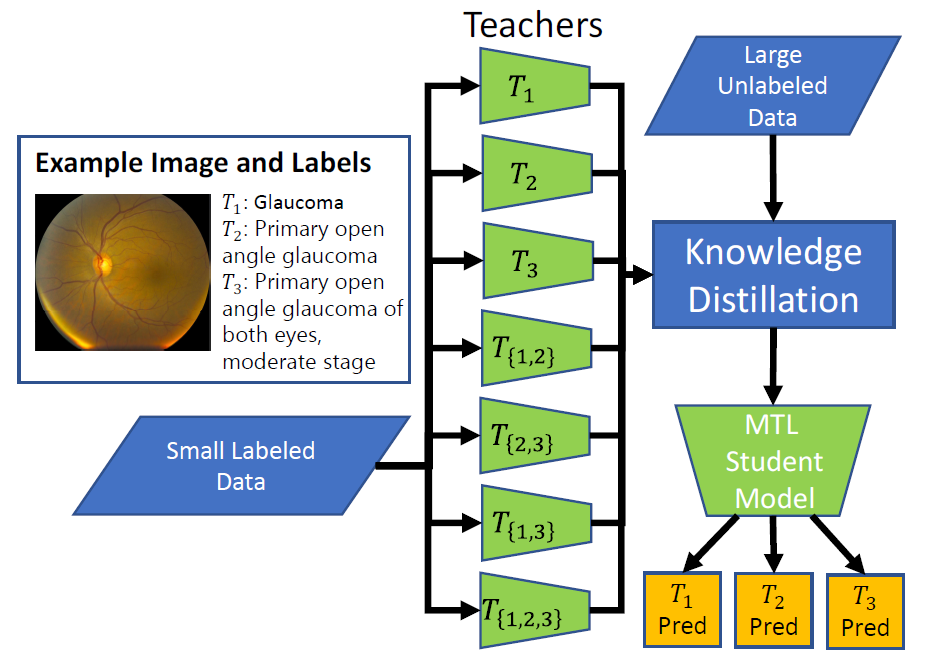
\includegraphics[width=0.8\textwidth]{Archi.PNG}
\end{frame}



\section{Literature Review}
\begin{frame}{Literature Review}
    \begin{itemize}
        \item Overviews of Computer Vision application in the medical field  \cite{OverviewMedical1} and \cite{OverviewMedical2}
        \item Multi Task Learning: first article on the topic  \cite{Multitask1}. Current day overview and a glimpse into the future \cite{Multitask2}.
        \item Survey covering knowledge distilation \cite{KD1} from many different perspectives and approaches.
        \item First papers on combinations of these transfer learning methods appear around 2016. \cite{MTKD2} propose another approach to this problem and \cite{MTKD1} propose usage of those methods in NLP task.
    \end{itemize}
\end{frame}



\section{Division of work}
\begin{frame}{Division of work}
\begin{itemize}
    \item Selecting datasets
    \item Data processing
    \item Creating MTL teachers models
    \item Distill knowledge to student model
    \item Evaluate results
\end{itemize}
\end{frame}

\section{Software and data}
\begin{frame}{Software and data}
Software:
\begin{itemize}
    \item PyTorch and Jupyter Notebooks - neural network development and data processing
    \item GitHub - code versioning and collaboration
    \item Google Colab - neural network training
\end{itemize}
Data:
\begin{itemize}
    \item Fundus images from paper
    \item Chest x-ray
    \item CT scans
\end{itemize}

\end{frame}

\section{Experiments}
\begin{frame}{Planned Experiments}
   Testing datasets from different background, as in medical and from another field.\\
   Comparing results from this architecture to baseline models and further testing, experiments depending on the implementation results.
\end{frame}

    

\begin{frame} [allowframebreaks]\frametitle{References}
               
        \bibliographystyle{apalike}
        \bibliography{bibfile}
\end{frame}

\end{document}